% Main ThesisTemplate ECE / AEE %
%
% Created by Mayer Florian October/2016
% v1.0
%
% October 2016: All packages are running 
% November 2017: Added more features: Bash-Code, corrected titlepage, listings, added ECM and Company Mode
% January 2020: More detailed options for titlepage, renewed design
% November 2020: Added Report-Titlepage and other degree programs, added some fixes

%%%%%%%%%%%%%%%%%%%%%%%%%%%%%%
\newcommand{\ECE}{1}
\newcommand{\ECM}{2}
\newcommand{\STM}{3}
\newcommand{\MEC}{4}
\newcommand{\Thesis}{1}
\newcommand{\Report}{3} 					%TODO
\newcommand{\PDF}{openany}
\newcommand{\Book}{openright}

\newcommand{\normalStyle}{1}
\newcommand{\FlowStyle}{3586}



%%%%%%%%%%%%%% A Way to add page labels to each page %%%%



%%%%% SOME OPTIONS %%%%% 
\newcommand{\german}{false} % germanTrue or false --> Switch between german and english headers / titlepage
\newcommand{\coloredTitlePage}{false} %false Switch between colored and BW titlepage
\newcommand{\company}{false}
\newcommand{\DocType}{\Thesis} %\Thesis \Report
\newcommand{\DegProg}{\STM}	%\ECE \ECM \STM \MEC
\newcommand{\Style}{\PDF}	%\PDF \Book
\newcommand{\FancyFactor}{\normalStyle}	%EasterEgg
%%%%% Required Settings for the template %%%%%
%%%%% Configuration Package for the ThesisTemplate ECE / ECM %%%%%%
%
% Created by Mayer Florian October/2016
% v1.0

%======= DocumentClass ===========%
\documentclass[11pt,\Style]{book} %Extarticle supports more FontSizes

%========= ADD Latex PACKAGES =========%
\usepackage[%
headtopline,plainheadtopline,% activate all lines (header and footer)
headsepline,plainheadsepline,%
footsepline,plainfootsepline,%
footbotline,plainfootbotline% auto update \..mark
]{scrlayer-scrpage}% (KOMA)

%\usepackage[utf8]{inputenc} %to allow vowel mutations
\usepackage{courier}
\renewcommand*\familydefault{\ttdefault} %% Only if the base font of the document is to be typewriter style
\usepackage[T1]{fontenc}
\usepackage{tikz} % Schematic creator with TikZ in LaTex
\usepackage{layout, geometry, titletoc} %geometry
\usepackage{float}
\usepackage{titlesec}
\usepackage{color, xcolor,colortbl}
\usepackage{graphicx,rotating}
\usepackage{nameref}

\usepackage{ifpdf}
\ifpdf
\usepackage{epstopdf}
\fi

\usepackage{lmodern}
\usepackage[titles]{tocloft}
\usepackage{blindtext}
\usepackage{anyfontsize}
\usepackage{setspace,varwidth}
\usepackage{ifthen}
\usepackage{multicol,multirow}
\usepackage{makecell}
\usepackage{shadowtext}
\usepackage{shadow}
\usepackage{contour}
\usepackage{hyphenat} %%Prevent hyphenates if wanted

\usepackage[final]{listings}% program code listings

\usepackage{amssymb}
\usepackage{emptypage}
\usepackage{glossaries}
\usepackage{appendix}
\usepackage{mdframed}
\usepackage{etoolbox}
\usepackage{chngcntr}
\usepackage{beramono} 

\usepackage{textcomp}
\usepackage[european,RPvoltages]{circuitikz}
%\usepackage{footmisc}% customize footnotes
\usepackage[%
% allow line break in links
colorlinks=true,% if false: framed link
linkcolor=black,anchorcolor=black,citecolor=black,filecolor=black,%
menucolor=black,urlcolor=black]{hyperref}% hyperlinks for references
\usepackage[nameinlink,noabbrev]{cleveref} % Provides support for clever references.

\ifthenelse{\equal{\german}{true}}
{
	\usepackage[ngerman]{babel}
	\renewcommand{\lstlistlistingname}{Programmcode}
}
{
	\usepackage[american]{babel}
}
\usepackage{accsupp}
\newcommand{\noncopynumber}[1]{%
	\BeginAccSupp{method=escape,ActualText={}}%
	#1%
	\EndAccSupp{}%
}
%========= ADD TikZ PACKAGES =========%
\usetikzlibrary{matrix,calc,positioning,arrows,shapes}
\usetikzlibrary{decorations.pathreplacing}

\ifthenelse{\equal{\Style}{\Book}}
{
	\geometry{a4paper,twoside,%
		%textheight=205mm, %246mm,%
		textwidth=165mm,%
		top = 3cm,
		bottom = 4cm,
		heightrounded=false,% round textheight to multiple of lines (avoids overfull vboxes)
		ignoreall=true,% do not include header, footer, and margins in calculations
		marginparsep=5pt,% marginpar only used for signs (centered), thus only small sep. needed
		marginparwidth=10mm,% prevent margin notes to be out of page
		hmarginratio=1:2,
		voffset = 2.25mm,
		%headheight = 16mm,
		headsep = 9mm,
		footskip = 13mm
	}
}
{
	\geometry{a4paper,%
	%textheight=205mm, %246mm,%
	textwidth=165mm,%
	top = 3cm,
	bottom = 4.25cm,
	left = 2.25cm,
	heightrounded=false,% round textheight to multiple of lines (avoids overfull vboxes)
	ignoreall=true,% do not include header, footer, and margins in calculations
	marginparsep=0pt,% marginpar only used for signs (centered), thus only small sep. needed
	marginparwidth=0mm,% prevent margin notes to be out of page
	hmarginratio=1:2,
	voffset = 2.25mm,
	%headheight = 16mm,
	headsep = 9mm,
	footskip = 13mm
	}
}

%%%%%% Correct Even and Odd Pages %%%%%
\let\tmp\oddsidemargin
\let\oddsidemargin\evensidemargin
\let\evensidemargin\tmp
\reversemarginpar

\linespread{1.4}
%======= DEFINE COLORS ===========%
\definecolor{DENcol}{RGB}{35,171,196} % Department Colour
\definecolor{DENcolDark}{RGB}{28,136,156} % Department DarkColour
\definecolor{commentsColor}{rgb}{0.497495, 0.497587, 0.497464}
\definecolor{keywordsColor}{RGB}{35,171,196}
\definecolor{stringColor}{rgb}{0.558215, 0.000000, 0.135316}

\definecolor{mybluei}{RGB}{0,173,239}
\definecolor{myblueii}{RGB}{63,200,244}
\definecolor{myblueiii}{RGB}{199,234,253}

%======= Re-Define Essential Commands and store old ones ======%
\newcommand{\ChapterFont}{qag}
\ifthenelse{\equal{\FancyFactor}{\FlowStyle}}
{
	\newcommand{\WorkingFont}{\sfdefault}
}
{
	\newcommand{\WorkingFont}{\rmdefault}
}
\renewcommand{\familydefault}{\WorkingFont}
\normalfont

%======= Set Depths of TOC / TOF / TOL =======%
\renewcommand{\cftchapfont}{\bf\large\fontfamily{\sfdefault}\selectfont}
\renewcommand{\cftpartfont}{\bf\large\fontfamily{\sfdefault}\selectfont}

%====== Usefull Additional Commands =======%
\newcommand{\ie}{i.\,e.}
\newcommand{\Ie}{I.\,e.}
\newcommand{\eg}{e.\,g.}
\newcommand{\Eg}{E.\,g.} 

%====== Heading Commands =======%
\renewcommand*\chaptermark[1]{\markleft{\thechapter~#1}}
\renewcommand*\sectionmark[1]{\markright{\thesection~#1}}

\ihead[]{}
\ohead[\ShortTitle]{\footnotesize\headmark}%


\ifthenelse{\equal{\Style}{\Book}}
{
	\ofoot[\ifthenelse{\equal{\thepage}{}}{\pagemark}{--~~\pagemark~~--}]{\ifthenelse{\equal{\thepage}{}}{\pagemark}{--~~\pagemark~~--}}%
	\cfoot[]{}%
}
{
	\cfoot[\ifthenelse{\equal{\thepage}{}}{\pagemark}{--~~\pagemark~~--}]{\ifthenelse{\equal{\thepage}{}}{\pagemark}{--~~\pagemark~~--}}%
	\ofoot[]{}%
}

%============== Chapter / Section / Subsection Style ==== %
\newcommand{\resumecontentsFlow}{
	\ifthenelse{\equal{\FancyFactor}{\FlowStyle}}
	{
		\resumecontents
	}
	{
	}
}
\newcommand{\stopcontentsFlow}{
	\ifthenelse{\equal{\FancyFactor}{\FlowStyle}}
	{
		\stopcontents
	}
	{
	}
}


\titleformat{\chapter}[display]
{\sffamily\bfseries\fontsize{22}{22}\selectfont}%\
{
	\begin{tikzpicture}[overlay]
		\node (CoolTitle) at (11.75,1.75) [opacity=0.325]{\includegraphics[scale=0.85]{temp_graphics/chapterBacking.eps}};
		\node (titleNumber) at ($(CoolTitle)+(3,0)$) {\textcolor{black!80}{\fontfamily{\ChapterFont}\bfseries\Large\fontsize{80}{80}\selectfont\thechapter}};
	\end{tikzpicture}
}
{0.05em}%
{\vspace{0.25ex}\filleft}%
%
\titleformat{\section}{\Large \bfseries \sffamily}{\thesection}{1 em}{}
\titleformat{\subsection}{\large \bf \sffamily}{\thesubsection}{1 em}{}
\titleformat{\subsubsection}{\large \bf \sffamily}{\thesubsubsection}{1 em}{}

\newcommand\partnumfont{% font specification for the number
	\fontsize{200}{75}\color{DENcolDark!40}\selectfont\sffamily%
}

\newcommand\partnamefont{% font specification for the name "PART"
	\fontsize{45}{45}\color{DENcolDark!40}\selectfont\sffamily 
}

\titleformat{\part}[display]
{\sffamily\bfseries\fontsize{35}{35}\selectfont\color{black!75}\thispagestyle{empty}
}%\
{	
	\ifthenelse{\equal{\FancyFactor}{\FlowStyle}}
	{
	\begin{tikzpicture}[overlay]
		\node (PartBacking) at (current page.south west) [rectangle,minimum width=40cm, minimum height=40cm, fill=DENcol!10]{};
		\node [rectangle, text width= 10cm, align = right] (titleNumber) at ($(PartBacking)+(12.125,3.5)$) {\partnumfont\thepart};
		\node (titleName) at ($(titleNumber)+(2.25,3.5)$) {\partnamefont PART};	
		\node [rounded corners=10pt, fill = white, text opacity=1, fill opacity=0.5] (miniTOC) at (9.25,-11) {
			\startcontents
			\stopcontents
			\begin{minipage}{14cm}		
				\singlespacing\thispagestyle{empty}\fontsize{12}{12}\printcontents{}{0}[1]{}
			\end{minipage}};	
	\end{tikzpicture}
	}
	{
	\begin{tikzpicture}[overlay]
		\node (PartBacking) at (current page.south west) [rectangle,minimum width=40cm, minimum height=40cm, fill=DENcol!10]{};
		\node [rectangle, text width= 10cm, align = right] (titleNumber) at ($(PartBacking)+(12.125,3.5)$) {\partnumfont\thepart};
		\node (titleName) at ($(titleNumber)+(2.25,3.5)$) {\partnamefont PART};	
	\end{tikzpicture}
	}{}
}
{0.05em}%
{\vspace{0.25ex}\filleft}

%%%%% TOC Costumizations %%%%%%
\contentsmargin{0cm} % Removes the default right margin

%------------------------------------------------

% Styling of numbered parts in the table of contents
\newcommand{\tocentrypartnumbered}[1]{%
	\setlength\fboxsep{0pt}% Remove box padding
	\contentslabel[%
	% Part number box
	\colorbox{DENcol!10}{% Background color
		\strut\parbox[c][.7cm]{1.1cm}{% Box size
			\color{DENcol!70}\Large\sffamily\bfseries\centering\thecontentslabel% Part number
		}%
	}%
	\hspace{4pt}%
	% Part title box
	\colorbox{DENcol!10}{% Background color
		\strut\parbox[c][.7cm]{\linewidth-1.25cm}{% Box size
			\centering\Large\sffamily #1% Part title
		}%
	}%
	]{1.25cm}
}

% Styling of unnumbered parts in the table of contents
\newcommand{\tocentrypartunnumbered}[1]{%
	\setlength\fboxsep{0pt}% Remove box padding
	\contentslabel[%
	% Part title box
	\colorbox{DENcol!10}{% Background color
		\strut\parbox[c][0.7cm]{\linewidth}{% Box size
			\centering\LARGE\sffamily #1 % Part title
		}%
	}%
	]{1.25cm}
}

% New Page Style
\newcommand{\emptydoublepage}{%
  \newpage{\pagestyle{empty}\cleardoublepage}
}


\titlecontents{part} % Section type being modified
[1.25cm] % Left indentation
{\addvspace{0pt}\Large\sffamily\bfseries\hypersetup{linkcolor=black}} % Before code
{\tocentrypartnumbered} % Formatting of numbered sections of this type
{\tocentrypartunnumbered} % Formatting of numberless sections of this type
{} % Formatting of the filler to the right of the heading and the page number
[] % After code

%------------------------------------------------

\titlecontents{chapter} % Section type being modified
[1.3cm] % Left indentation
{\addvspace{12pt}\Large\sffamily\bfseries\hypersetup{linkcolor=DENcolDark!90}} % Before code
{\bfseries\color{DENcol}\contentslabel[\Large\thecontentslabel]{1.25cm}} % Formatting of numbered sections of this type
{} % Formatting of numberless sections of this type
{\color{DENcol!75}\normalsize\;\titlerule*[6pt]{.}\;\color{DENcol}\thecontentspage} % Formatting of the filler to the right of the heading and the page number
[] % After code

%------------------------------------------------

% code listings
\newcommand\realnumberstyle[1]{}

\makeatletter
\newcommand{\zebra}[3]{%
	{\realnumberstyle{#3}}%
	\begingroup
	\lst@basicstyle
	\ifodd\value{lstnumber}%
	\color{#1}%
	\else
	\color{#2}%
	\fi
	\rlap{\hspace*{\lst@numbersep}%
		\color@block{\linewidth}{\ht\strutbox}{\dp\strutbox}%
	}%
	\endgroup
}
\makeatother

\lstloadlanguages{Bash,VHDL,Matlab,[ANSI]C,Java,[LaTeX]TeX,Python}

\lstset{
	frame=top,frame=bottom,
	basicstyle=\fontsize{9}{9}\ttfamily, %fontsize{8}{8}\normalfont,    % the size of the fonts that are used for the code
	stepnumber=1,                           % the step between two line-numbers. If it is 1 each line will be numbered
	numbersep=13pt,                         % how far the line-numbers are from the code
	tabsize=3,                              % tab size in blank spaces
	extendedchars=true,                     %
	breaklines=true,                        % sets automatic line breaking
	captionpos=t,                           % sets the caption-position to top
	columns=fullflexible,
	mathescape= false,
	numberstyle=\fontsize{7}{7}\ttfamily\zebra{black!10}{black!2}{}\noncopynumber,
	numbers = left, 
	keywordstyle=\color{keywordsColor}\bfseries,
	stringstyle=\color{stringColor}\ttfamily, % Farbe der String
	commentstyle=\color{commentsColor}\textit,
	showspaces=false,           % Leerzeichen anzeigen ?
	showtabs=false,             % Tabs anzeigen ?
	xleftmargin=15pt,
	framexleftmargin=14pt,
	framexrightmargin=9pt,
	framexbottommargin=5pt,
	framextopmargin=5pt,
	showstringspaces=false,      % Leerzeichen in Strings anzeigen ?
	linewidth = 150mm
}

%%%% MDBOX Setup
\mdfsetup{%
	middlelinecolor=red,
	middlelinewidth=2pt,
	backgroundcolor=black!5,
	roundcorner=40pt,
	topline = false,
	bottomline = false,
	rightline = false,
	linecolor = DENcol!45,
	linewidth = 6pt}

%%%% GET RID OF OVERFULL BOXING WARNINGS %%%%
%\overfullrule=5pt
\setlength{\headheight}{1.1\baselineskip}
\raggedbottom

%%%%%%%%%%%%%
\counterwithout{footnote}{chapter}

\makeglossaries

\begin{document}
%%%% Now we include the glossaries %%%%	
%%%%% ThesisTemplate ECE / AEE %%%%%%
%
% Created by Mayer Florian October/2016
% v1.0

%============== Glossary Command ==== %

\newglossaryentry{SCSS}{name=SCSS, description={Single Channel Source Separation}} 
\newglossaryentry{ITD}{name=ITD, description={Interaural Time Difference}}
\newglossaryentry{PASCSS}{name=PASCSS, description={Phase-Aware Single Channel Source Separation}}
\newglossaryentry{CASA}{name=CASA, description={Computational Auditory Scene Analysis}}
\newglossaryentry{NMF}{name=NMF, description={Non-Negative Matrix Factorization}}
\newglossaryentry{CMF}{name=CMF, description={Complex Matrix Factorization}}
\newglossaryentry{STFT}{name=STFT, description={Short-Time Fourier Transformation}}
\newglossaryentry{DTFT}{name=DTFT, description={Discrete-Time Fourier Transformation}}
\newglossaryentry{ISTFT}{name=ISTFT, description={Inverse Short-Time Fourier Transformation}}
\newglossaryentry{IBM}{name=IBM, description={Ideal Binary Mask}}
\newglossaryentry{IRM}{name=IRM, description={Ideal Ratio Mask}}
\newglossaryentry{SNR}{name=SNR, description={Signal-to-Noise Ratio}}
\newglossaryentry{DNN}{name=DNN, description={Deep neural network}}
\newglossaryentry{SVM}{name=SVM, description={Support vector machine}}
\newglossaryentry{KL-divergence}{name=KL-divergence, description={Kullback-Leibler divergence}}
\newglossaryentry{MPE}{name=MPE, description={Multipitch Estimator}} 
\newglossaryentry{PEFAC}{name=PEFAC, description={Pitch Estimation Filter with Amplitude Compression}}  
\newglossaryentry{GMM}{name=GMM, description={Gaussian mixture models}} 
\newglossaryentry{GLA}{name=GLA, description={Griffin and Lim Algorithm}}  
\newglossaryentry{MISI}{name=MISI, description={Multiple Input Spectrogram Inversion}}
\newglossaryentry{PPR}{name=PPR, description={Partial Phase Reconstruction}}
\newglossaryentry{ISSIR}{name=ISSIR, description={Partial Phase Reconstruction for Informed Source Separation}}
\newglossaryentry{FHMM}{name=FHMM, description={Factorial Hidden Markov Models}}
\newglossaryentry{HMM}{name=HMM, description={Hidden Markov Models}}
\newglossaryentry{SHR}{name=SHR, description={Subharmonic to harmonic ratio}}
\newglossaryentry{POC}{name=POC, description={Proof of Concept}}
\newglossaryentry{SSR}{name=SSR, description={Signal-to-Signal Ratio}}
\newglossaryentry{GPE}{name=GPE, description={Gross-Pitch Error}}
\newglossaryentry{MMSE}{name=MMSE, description={Minimum Mean Squared Error}}
\newglossaryentry{PESQ}{name=PESQ, description={Perceptual Evaluation of Speech Quality}}
\newglossaryentry{STOI}{name=STOI, description={Short-time objective intelligibility}}
\newglossaryentry{BSS-Eval}{name=BSS-Eval, description={Blind Source separation evaluation}}
\newglossaryentry{SDR}{name=SDR, description={Signal-to-Distortion Ratio}}
\newglossaryentry{SIR}{name=SIR, description={Signal-to-Interference Ratio}}
\newglossaryentry{SAR}{name=SAR, description={Signal-to-Artifact Ratio}}
\newglossaryentry{PE}{name=PE, description={Phase Estimation}}
\newglossaryentry{SSN}{name=SSN, description={Speech-Shaped Noise}}
% in order to compile your glossaries you need to call \makeglossaries in your compiling-chain as well
%%%%%%%%%%%%	

%frontmatter inluding: titlepage, abstract, acknowledgments, declaration, toc, lof, lot
\frontmatter
\renewcommand{\thepage}{\Roman{page}}

%%%% Modify your titlepage by configuring "frontmatter/tpThesis.tex" or "frontmatter/tpReport.tex"
%%% BEGIN FRONTMATTER
%%%% Modify your titlepage by configuring "frontmatter/tpThesis.tex" or "frontmatter/tpReport.tex"
%%% BEGIN FRONTMATTER
\ifthenelse{\equal{\DocType}{\Thesis}}
{
	\newcommand{\ThesisTitle}{Title of your Thesis} %Title of your Thesis
\newcommand{\ThesisSubtitle}{Additional Title} %Additional Title
\newcommand{\ShortTitle}{Short Title of your Thesis} %Short Title of your Thesis
\newcommand{\ThesisAuthor}{Author} %Author 

\newcommand{\Supervisor}{Supervisor} % Supervisor 1 \\ Supervisor 2 \\ ...

\newcommand{\CoSupervisor}{Ihr externer Betreuer} % Supervisor 1 \\ Supervisor 2 \\ ...
\newcommand{\Assessors}{Prüfer Eins \\ Prüfer Zwei \\ weitere....} % Your Assessors 
\newcommand{\SpecialNote}{}
	
\begin{titlepage}
    \centering
    \vspace*{1cm}
    
    \Huge
    \textbf{Deep Learning Architectures}
    
    \vspace{0.5cm}
    \LARGE
    A Comprehensive Overview and Guide
    
    \vspace{1.5cm}
    
    \textbf{Your Name}
    
    \vfill
    
    This document presents a detailed exploration \\
    of various deep learning architectures, \\
    their implementations, and applications. \\
    The Document was written using ChatGPT.
    
    \vspace{0.8cm}
    
    \Large
    FH JOANNEUM GmbH\\
    System Test Engineering\\
    Graz\\
    \today
    
    \vspace{2cm}
    
    
\includegraphics[width=0.4\textwidth]{figures/logo_fhj_stm.jpg}
    
    \vspace{3cm}
\end{titlepage}

	\newpage	
	%%%%% ThesisTemplate ECE / AEE %%%%%%
%
% Created by Mayer Florian October/2016
% v1.0

% English
%\ifthenelse{\equal{\DocumentLanguage}{en}}{

% \ifthenelse{\equal{\DocumentLanguage}{de}}{
	\thispagestyle{empty}
	{\hfill\fontfamily{\sfdefault}\bfseries\fontsize{22}{22}\selectfont{Obligatory declaration}}\vspace*{1cm}
	
	\noindent I hereby confirm and declare that the present \DocTypeText ~was composed by myself without any help from others and that the work contained herein is my own and that I have only used the specified sources and aids. The uploaded version is identical to any printed version submitted.
	
	\noindent I also confirm that I have prepared this thesis in compliance with the principles of the \nohyphens{FH JOANNEUM} Guideline for Good Scientific Practice and Prevention of Research Misconduct.
	
	\noindent I declare in particular that I have marked all content taken verbatim or in substance from third party works or my own works according to the rules of good scientific practice and that I have included clear references to all sources.\\
	\noindent The present original thesis has not been submitted to another university in Austria or abroad for the award of an academic degree in this form.
	I understand that the provision of incorrect information in this signed declaration may have legal consequences.
	
	\ifthenelse{\equal{\Style}{\Book}}
	{
		\newpage
		\thispagestyle{empty}	
	}
	
%	\par\vspace*{4cm}
%	\centerline{
%	\begin{tabular}{m{1.5cm}cm{1.5cm}m{3cm}m{1.5cm}cm{1.5cm}}
%	\cline{1-3} \cline{5-7}
%	& Date & & & & (Signature) &\\
%	\end{tabular}}
% }

	\ifthenelse{\equal{\DegProg}{\ECE}}
	{
		%%%%% ThesisTemplate ECE / AEE %%%%%%
%
% Created by Mayer Florian October/2016
% v1.0
\newpage
\thispagestyle{empty} \vspace*{1cm}

{\hfill\fontfamily{\sfdefault}\bfseries\fontsize{22}{22}\selectfont{Kurzfassung}} \vspace*{1cm}

\noindent 
Hier sollte Ihre Zusammenfassung der Arbeit stehen!

\ifthenelse{\equal{\Style}{\Book}}
{
	\newpage\null\thispagestyle{empty}\newpage
}
{
}
	}{}	
	\newpage
	%%%%% ThesisTemplate ECE / AEE %%%%%%
%
% Created by Mayer Florian October/2016
% v1.0

\thispagestyle{empty} \vspace*{1cm}

{\hfill\fontfamily{\sfdefault}\bfseries\fontsize{22}{22}\selectfont{Abstract}} \vspace*{1cm}

\noindent 
Please put the summary of your work here! 

	%%%%% ThesisTemplate ECE / AEE %%%%%%
%
% Created by Mayer Florian October/2016
% v1.0

\newpage
\thispagestyle{empty} \vspace*{1cm}

% English
%\ifthenelse{\equal{\DocumentLanguage}{en}}{
{\hfill\fontfamily{\sfdefault}\bfseries\fontsize{22}{22}\selectfont{Acknowledgments}} \vspace*{1cm}

\noindent 
Thanks to .....


\vspace*{5cm} %You could also add "\newpage" here ! Choose whatever suits you best



	%%%%%% ThesisTemplate ECE / AEE %%%%%%
%
% Created by Mayer Florian October/2016
% v1.0

%============== Glossary Command ==== %

\newglossaryentry{SCSS}{name=SCSS, description={Single Channel Source Separation}} 
\newglossaryentry{ITD}{name=ITD, description={Interaural Time Difference}}
\newglossaryentry{PASCSS}{name=PASCSS, description={Phase-Aware Single Channel Source Separation}}
\newglossaryentry{CASA}{name=CASA, description={Computational Auditory Scene Analysis}}
\newglossaryentry{NMF}{name=NMF, description={Non-Negative Matrix Factorization}}
\newglossaryentry{CMF}{name=CMF, description={Complex Matrix Factorization}}
\newglossaryentry{STFT}{name=STFT, description={Short-Time Fourier Transformation}}
\newglossaryentry{DTFT}{name=DTFT, description={Discrete-Time Fourier Transformation}}
\newglossaryentry{ISTFT}{name=ISTFT, description={Inverse Short-Time Fourier Transformation}}
\newglossaryentry{IBM}{name=IBM, description={Ideal Binary Mask}}
\newglossaryentry{IRM}{name=IRM, description={Ideal Ratio Mask}}
\newglossaryentry{SNR}{name=SNR, description={Signal-to-Noise Ratio}}
\newglossaryentry{DNN}{name=DNN, description={Deep neural network}}
\newglossaryentry{SVM}{name=SVM, description={Support vector machine}}
\newglossaryentry{KL-divergence}{name=KL-divergence, description={Kullback-Leibler divergence}}
\newglossaryentry{MPE}{name=MPE, description={Multipitch Estimator}} 
\newglossaryentry{PEFAC}{name=PEFAC, description={Pitch Estimation Filter with Amplitude Compression}}  
\newglossaryentry{GMM}{name=GMM, description={Gaussian mixture models}} 
\newglossaryentry{GLA}{name=GLA, description={Griffin and Lim Algorithm}}  
\newglossaryentry{MISI}{name=MISI, description={Multiple Input Spectrogram Inversion}}
\newglossaryentry{PPR}{name=PPR, description={Partial Phase Reconstruction}}
\newglossaryentry{ISSIR}{name=ISSIR, description={Partial Phase Reconstruction for Informed Source Separation}}
\newglossaryentry{FHMM}{name=FHMM, description={Factorial Hidden Markov Models}}
\newglossaryentry{HMM}{name=HMM, description={Hidden Markov Models}}
\newglossaryentry{SHR}{name=SHR, description={Subharmonic to harmonic ratio}}
\newglossaryentry{POC}{name=POC, description={Proof of Concept}}
\newglossaryentry{SSR}{name=SSR, description={Signal-to-Signal Ratio}}
\newglossaryentry{GPE}{name=GPE, description={Gross-Pitch Error}}
\newglossaryentry{MMSE}{name=MMSE, description={Minimum Mean Squared Error}}
\newglossaryentry{PESQ}{name=PESQ, description={Perceptual Evaluation of Speech Quality}}
\newglossaryentry{STOI}{name=STOI, description={Short-time objective intelligibility}}
\newglossaryentry{BSS-Eval}{name=BSS-Eval, description={Blind Source separation evaluation}}
\newglossaryentry{SDR}{name=SDR, description={Signal-to-Distortion Ratio}}
\newglossaryentry{SIR}{name=SIR, description={Signal-to-Interference Ratio}}
\newglossaryentry{SAR}{name=SAR, description={Signal-to-Artifact Ratio}}
\newglossaryentry{PE}{name=PE, description={Phase Estimation}}
\newglossaryentry{SSN}{name=SSN, description={Speech-Shaped Noise}}
}
{
}
%%% END FRONTMATTER
%%% END FRONTMATTER
%By commenting the elements below, you directly deactivate the use of each of the elements as well
\tableofcontents
\listoffigures
\listoftables
\lstlistoflistings
\printglossary

\mainmatter %including: Parts, chapters, sections, appendicies
\renewcommand{\thepage}{\arabic{page}}

\chapter{Examples}\label{ch:Examples}
This Chapter contains examples of how to use the template with different elements, like images, tables, code, lists.
\section{Text}\label{sec:text}
This section is meant to show how to integrate text structured in section ans subsactions can be add to the document.

\subsection{Various Formatting Styles in Text}\label{subsec:formatting_styles_text}
Here is an example text that demonstrates various formatting styles:

\begin{itemize}
    \item \textbf{Bold text}
    \item \textit{Italic text}
    \item \underline{Underlined text}
    \item \texttt{Code text}
\end{itemize}

You can use these formatting styles to enhance the visual appearance of your text in your LaTeX document.

\section{Image Section}
\label{image_section}

% Section title slide
\sectiontitleframe{Image Section}

\begin{frame}{Image with Caption}
  \begin{figure}
    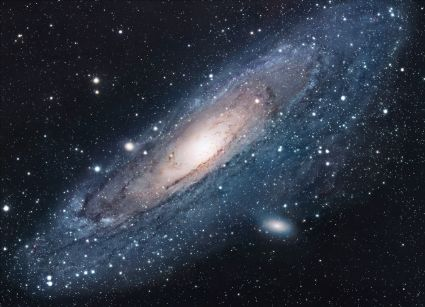
\includegraphics[width=0.7\textwidth]{figures/universe.jpg} % Replace 'example-image' with your image file
    \caption{This is a beautiful image.}
    \label{fig:sampleimage}
  \end{figure}
\end{frame}

\begin{frame}{Reference to the Image}
  In the previous frame, we saw a beautiful image (see Figure~\ref{fig:sampleimage}). It reminds us of the importance of visuals in our presentations.
\end{frame}
\newpage

\section{Table}\label{sec:table}
This section is meant to show how to integrate tables in the document.

\newcolumntype{M}{>{\centering\arraybackslash}p{0.7cm}}

\begin{table}[ht]
\centering
\begin{spacing}{1.1}\caption{Sample Table One}\label{table:tableOne}
\scriptsize
\begin{tabular}{|p{3.75cm}|M|M|M|M|M|M|M|M|M|M|}
\multicolumn{1}{c|}{\bf{}} &
\multicolumn{5}{c|}{\cellcolor{black!10}\bf{Gross-Pitch Error (GPE) (\%)}}  &
\multicolumn{5}{c|}{\cellcolor{black!10}\bf{Fine-Pitch Error (FPE) (Hz)}} \\
\hline
{GPE/FPE input signal} & \multicolumn{5}{c|}{{SNR (dB)}}  &
\multicolumn{5}{c|}{{SNR (dB)}} \\ \cline{2-6} \cline{7-11}
{} & {-6} & {-3} & {0} & {3} & {6} & {-6} & {-3} & {0} & {3} & {6} \\ \hline
{(UB): est. BM ({PEFAC})} & 26.07 & 23.67 & 21.10 & 19.41 & 18.56 & 0.71 & 0.59
& 0.75 & 0.63 & 0.69\\ \hline
{(UB): est. RM ({PEFAC})} & 25.16 & 22.29 & 18.51 & 18.62 & 16.54 & 0.71 & 0.63
& 0.79 & 0.74 & 0.88\\ \hline \hline
{est. BM ({PEFAC})} & 48.01 & 39.75 & 32.13 & 28.22 & 23.26 & 1.49 & 0.84
& 0.86 & 0.92 & 0.69\\ \hline
{est. BM ({proposed PE})} & 39.37 & 33.77 & 27.96 & 25.05 & 21.90 & 1.25 &
0.85 & 0.80 & 0.87 & 0.88\\ \hline
{est. RM ({PEFAC})} & 52.45 & 44.44 & 37.80 & 31.98 & 27.65 & 1.99 &
1.09 & 1.26 & 0.89 & 0.85\\ \hline
{est. RM ({proposed PE})} & 46.32 & 39.21 & 32.13 & 28.89 & 25.34 & 1.46 &
0.97 & 0.94 & 0.83 & 0.69\\ \hline \hline
{(LB): Mixed signal ({PEFAC})} & 66.2 & 60.55 & 53.98 & 46.52 & 40.33 & 2.96 & 2.42 & 2.22
& 1.71 & 1.46\\ \hline

\end{tabular}
\end{spacing}
\end{table}

\subsection{Reference to Table}\label{subsec:reference_table}
\noindent The Table of above is referenced here \cref{table:tableOne}.

\section{Python Code Section}
\label{python_code_section}
\sectiontitleframe{Python Code Section}

\begin{frame}[fragile]{Python Code Listing}
    \begin{lstlisting}[caption={Sample Python Code}, label=lst:pythoncode]
  from (*@\module{sklearn.preprocessing}@*) import (*@\class{PolynomialFeatures}@*)
 
  # This is a comment in Python
  def say_hello(name):
      print(f"Hello, {name}!")
  
  say_hello("world")
    \end{lstlisting}
  \end{frame}
  
  \begin{frame}{Reference to the Python Code}
    The Python function in Listing~\ref{lst:pythoncode} demonstrates a simple greeting.
  \end{frame}
  
\newpage
\section{Equation}\label{sec:equation}
This section is meant to show how to integrate equations in the document.

\begin{equation}\label{eq:example_equation}
	X(e^{j\omega})=\text{\gls{DTFT}T}\left(x(n)\right)=\sum_{n=-\infty}^{\infty}x(n)e^{-j\omega n},
\end{equation}

\noindent The equation above is referenced here \cref{eq:example_equation}.


\newpage
\section{List Structures}\label{sec:list_structures}
This section shows how to create different list structures.

\subsection{\emph{Itemize} create a bullet list}

\begin{itemize}
	\item First item
	\item Second item
	\item Third item
\end{itemize}

\subsection{\emph{Enumerate} create an enumerated list}

\begin{enumerate}
	\item First item
	\item Second item
	\item Third item
\end{enumerate}

\subsection{Nested lists}

\begin{enumerate}
	\item The first item
	\begin{enumerate}
		\item Nested item 1
		\item Nested item 2
	\end{enumerate}
	\item The second item
	\item The third etc \ldots
\end{enumerate}

 
\section{citations}
\label{sec:citations}
Here is a section with references to a book \citep{exampleBook}, a journal article \citep{exampleArticle}, a website \citep{exampleWebsite}, and a conference paper \citep{examplePaper}.


\chapter{Introduction}\label{ch:Introduction}

%
\newpage
\chapter{Methods}\label{ch:Methods}
\chapter{Results}\label{ch:Results}

\chapter{Discussion}\label{ch:Discussion}


%%%%  If necessary Appendicies %%%%%%%%%

\begin{appendices} % Put Appendicies here !! 
	% Section and Frames
\section*{Appendix}
\label{appendix_section}

% Section title frame
\sectiontitleframe{Appendix}

\begin{frame}[fragile]{Preprocessing Step Sequence Randomization I}
    \frametitle{Preprocessing Step Sequence Randomization I}
    \textbf{key points of the Sequence Randomization Feature:}
    \vspace{0.5em}
    \begin{itemize}
        \item A dynamic method to vary the order of preprocessing steps in image preprocessing pipelines.
        \item Preprocessing steps are probabilistically determined, allowing for varied combinations in the pipeline.
        \item Increases flexibility and efficiency in hyperparameter tuning.
    \end{itemize}
\end{frame}

\begin{frame}[fragile]{Preprocessing Step Sequence Randomization II}
    \frametitle{Preprocessing Step Sequence Randomization II}
    \begin{figure}
        \centering
        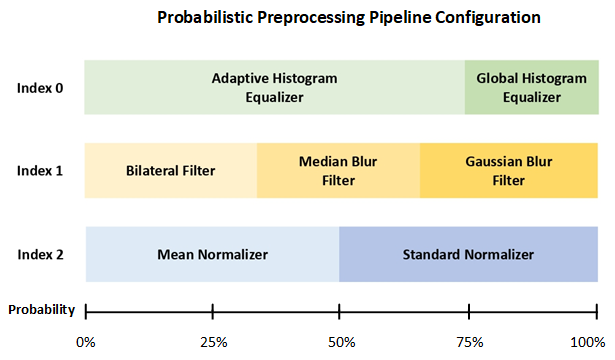
\includegraphics[width=0.8\textwidth]{figures/pipeline_sequence_randomisation_image.png}
        \caption{Illustration of the preprocessing step sequence randomization.}
    \end{figure}
\end{frame}

\begin{frame}[fragile]{Preprocessing Step Sequence Randomization III}
    \frametitle{Preprocessing Step Sequence Randomization III}
    \begin{lstlisting}[label=lst:probabilistic_pipeline_in_json, caption={Probabilistic Pipeline Sequence Definition in JSON Format.}, basicstyle=\scriptsize\ttfamily, stringstyle=\color{black}]
{
    "Adaptive Histogram Equalizer__I0F75": {...Parameters},
    
    "Global Histogram Equalizer__I0F25": {},

    "Bilateral Filter__I1F34": {...Parameters},

    "Median Blur Filter__I1F33": {...Parameters},

    "Gaussian Blur Filter__I1F33": {...Parameters},

    "Standard Normalizer__I2F50": {},

    "Mean Normalizer__I2F50": {},
}
    \end{lstlisting}
\end{frame}


	%\chapter*{Appendix B}
\addcontentsline{toc}{chapter}{Appendix B}

Appendix B could include extended tables, additional figures, or raw data relevant to your document. This section allows you to present all relevant material that supports your work but is too extensive to include in the main chapters.

\end{appendices} 


\ifthenelse{\equal{\german}{true}}
{
	\bibliographystyle{deIEEEtran}
}
{
	\bibliographystyle{IEEEtran}
}
	\bibliography{bib/STM_tempBib}

\end{document}